% !TEX root = ../../main.tex
% !TEX spellcheck = en_GB

\section{Modelling}
\label{sec:PureSineModelling}

The Matlab code for pitch shifting an input sine of \SI{470}{\hertz} is shown in \cref{app:matlabmodel}. It is primarily based on the description from Matlab \cite{MatlabIF} and the open source implementation in the Octave Signal package \cite{OctaveHilbert}.

\Cref{code:matlabmodel} shows pseudo code describing the Matlab model.
The blockSize is set, and a Hamming window is generated.
The window can be used for each block and it is only necessary to generate it once.
The phase starts at zero, but is updated after each loop, allowing for the next block to start with the correct phase shift.
The loop loads the samples, applies the window, finds the frequency, finds the closest C-major frequency, generates a sine at the correct frequency and phase and updates the phase.

\begin{listing}
	\begin{minted}[linenos, breaklines, bgcolor=lightgray]{matlab}
	blockSize = 512;
	h = hammingWindow(blockSize);
	phase = 0;
	
	while(1)
	y = load(blockSize);
	yh = h .* y;
	freqIn = findIF(yh);
	newFreq = pianoFreq(freqIn);
	[out, phase] = genSine(blockSize, newFreq);
	\end{minted}
	\caption{Pseudo code for the Matlab model.}
	\label{code:matlabmodel}
\end{listing}

Finding the frequency is done in five steps, the output of some plotted in \cref{fig:IFexplained}:
\begin{enumerate}
	\item Hilbert Transform
	\begin{itemize}
		\item Shifts the input signal by \ang{90}.
	\end{itemize}
	\item Determine the phase, \cref{fig:IFsub1}.
	\item Unwrap the phase, \cref{fig:IFsub2}.
	\item Calculate the derivative in each point, \cref{fig:IFsub3}.
	\item Calculate the mean of the middle portion of the points (in our case the middle third).
\end{enumerate}

The IF and phase is used to create a new sine.
This is done for each new block as shown in \cref{fig:IFoutput}.

\begin{figure}
	\centering
	\begin{subfigure}[t]{.5\textwidth}
		\centering
		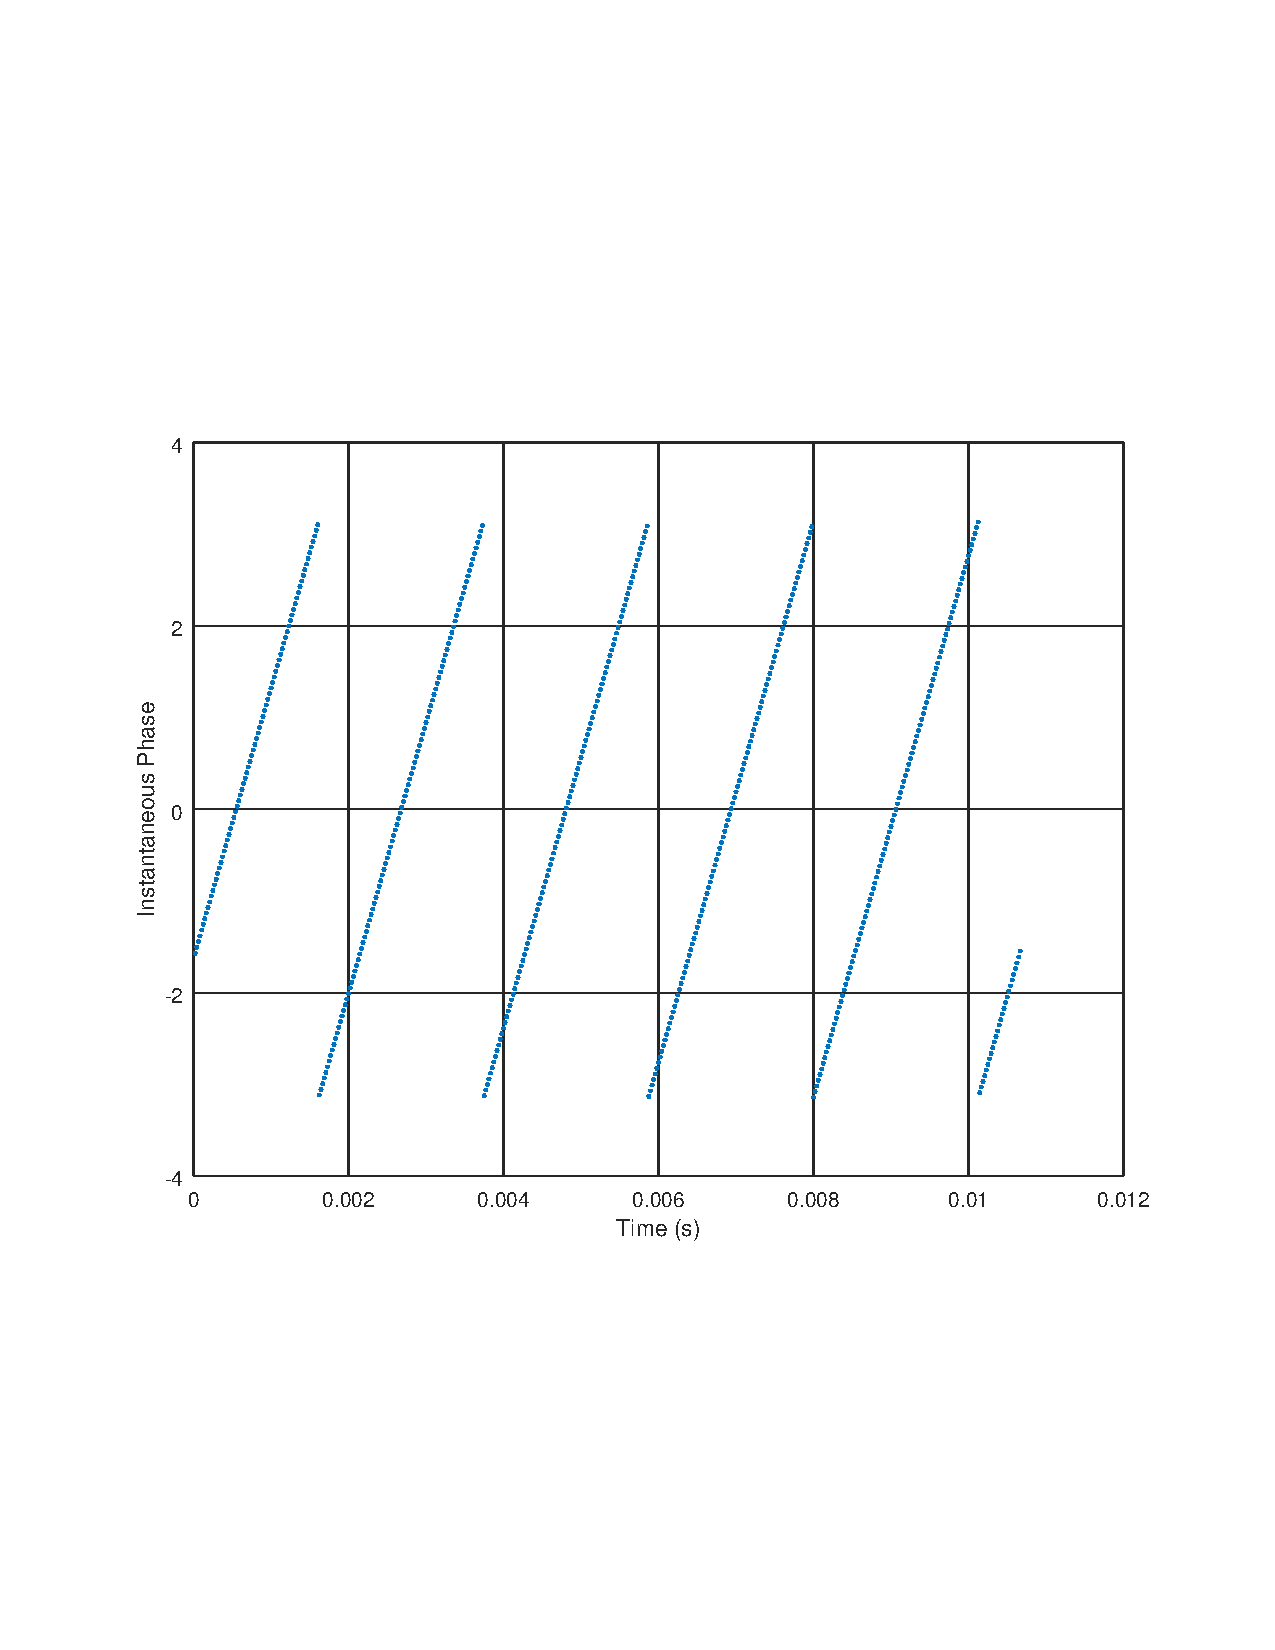
\includegraphics[width=.9\linewidth, clip, trim={2cm 7cm 2cm 7cm}]{gfx/Modelling/IFIP.pdf}
		\caption{Instantaneous Phase.}
		\label{fig:IFsub1}
	\end{subfigure}%
	\begin{subfigure}[t]{.5\textwidth}
		\centering
		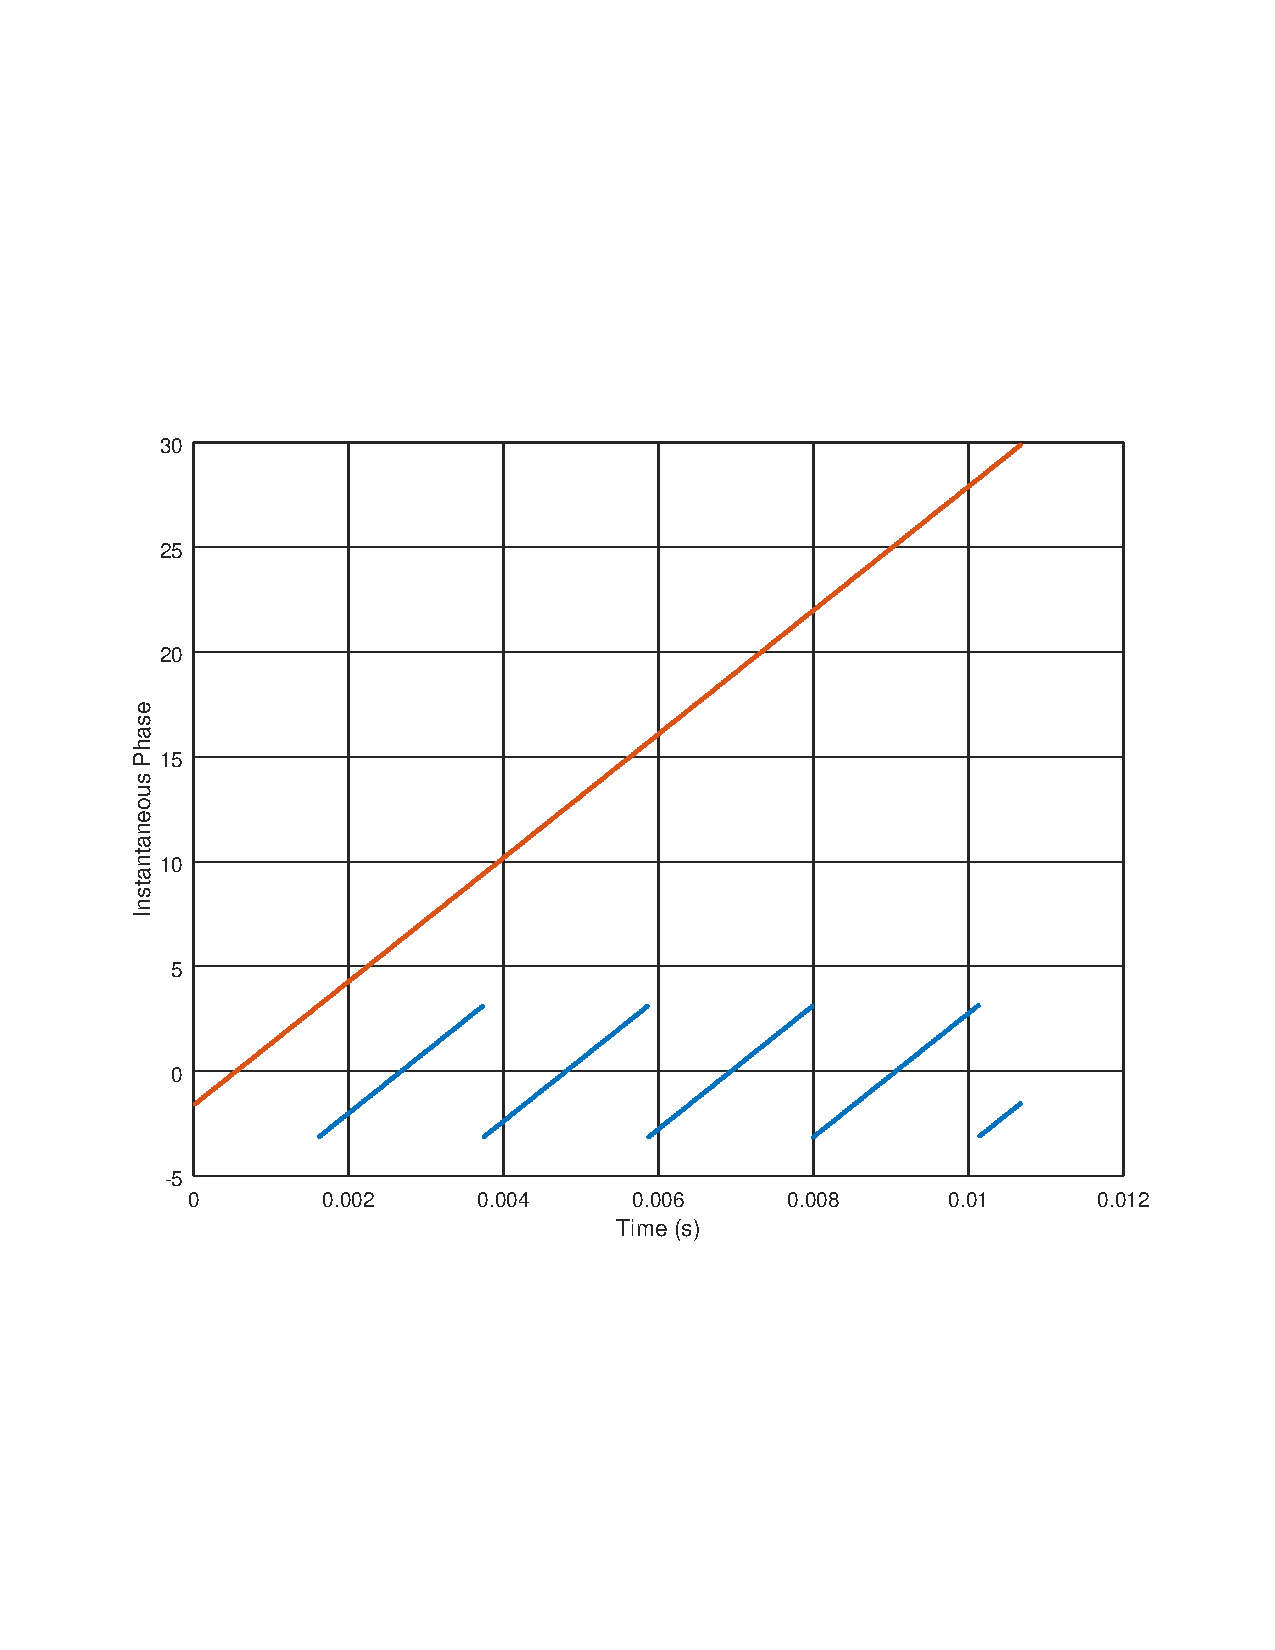
\includegraphics[width=.9\linewidth, clip, trim={2cm 7cm 2cm 7cm}]{gfx/Modelling/IFunwrap.pdf}
		\caption{Wrapping Instantaneous Phase (blue), and unwrapped Instantaneous Phase (red).}
		\label{fig:IFsub2}
	\end{subfigure} \\
	\begin{subfigure}[t]{.5\textwidth}
		\centering
		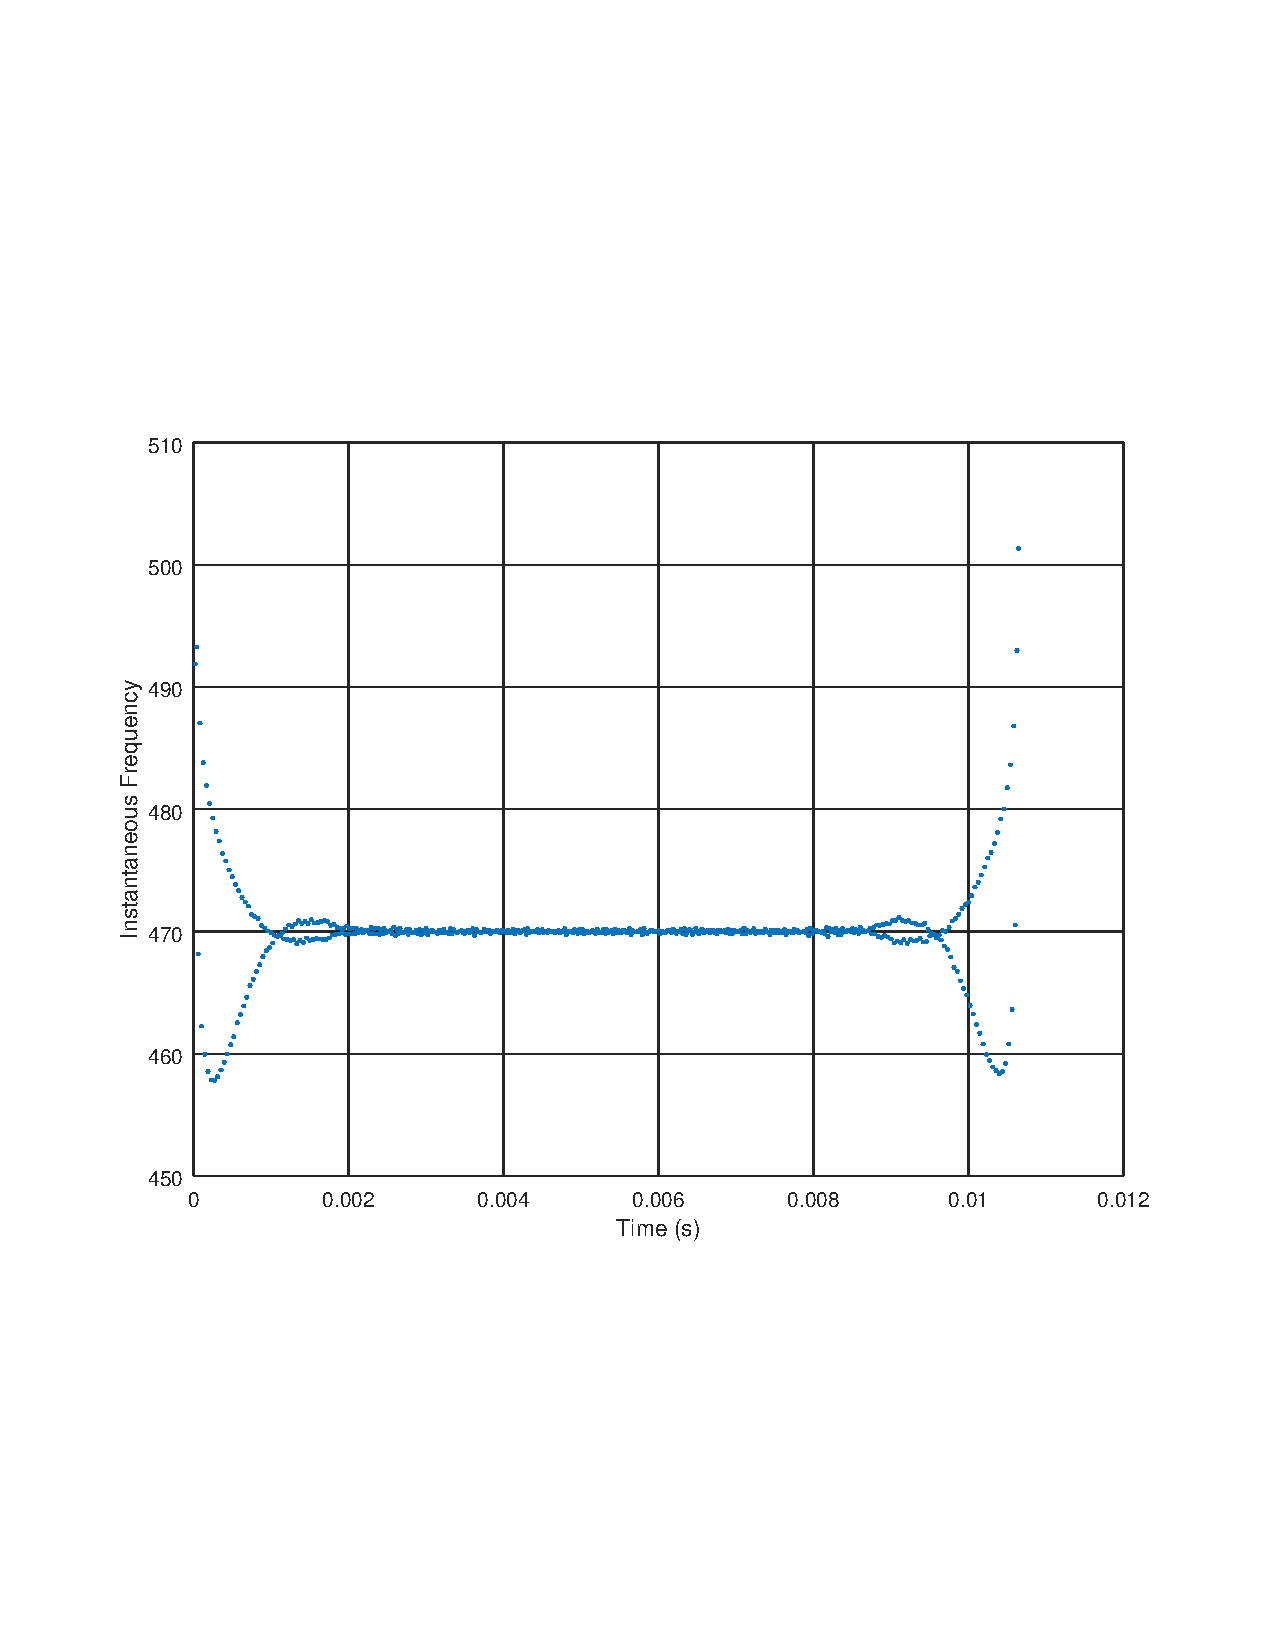
\includegraphics[width=.9\linewidth, clip, trim={2cm 7cm 2cm 7cm}]{gfx/Modelling/IFIF.pdf}
		\caption{Instantaneous Frequency. Derivative of the unwrapped phase.}
		\label{fig:IFsub3}
	\end{subfigure} 
	\caption{Different steps of determining the Instantaneous Frequency.}
	\label{fig:IFexplained}
\end{figure}

\begin{figure}
	\centering
	\begin{subfigure}[t]{.49\textwidth}
		\centering
		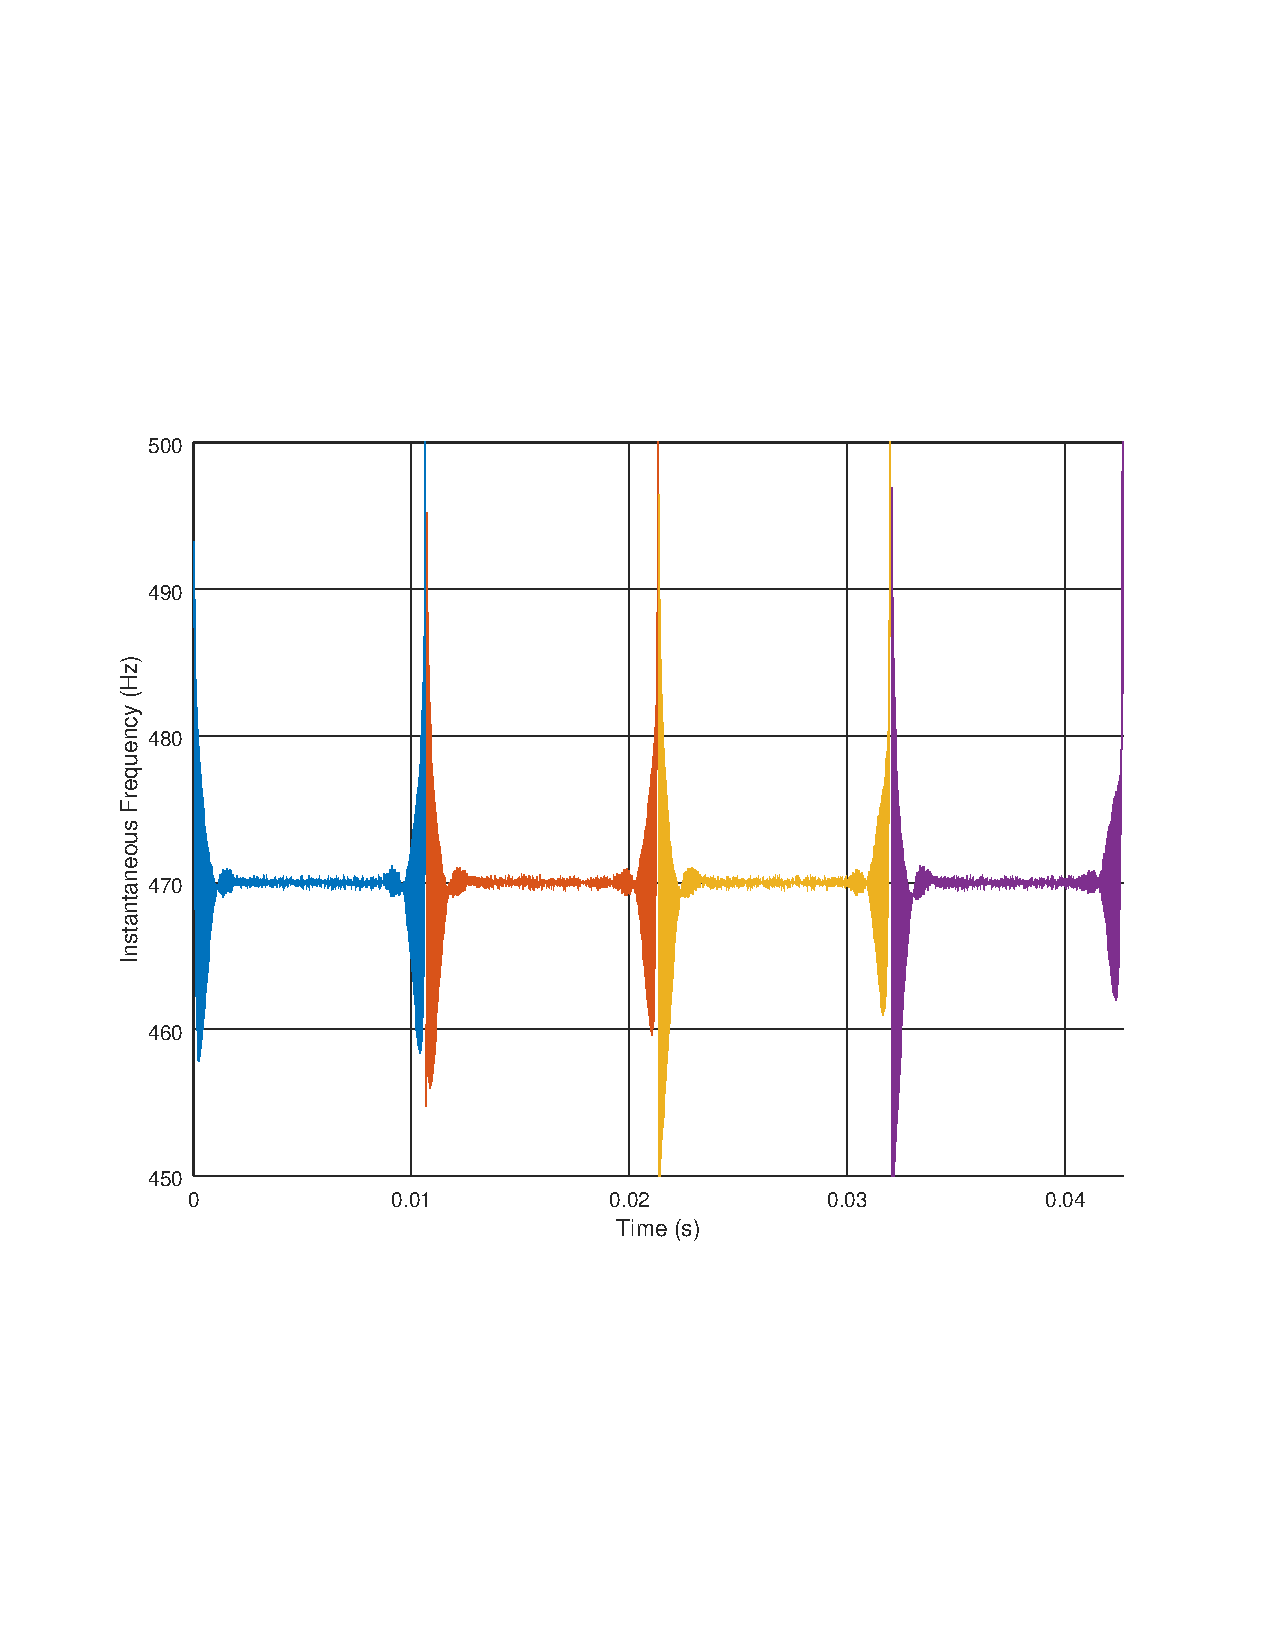
\includegraphics[width=.9\linewidth, clip, trim={2cm 7cm 2cm 7cm}]{gfx/Modelling/IF.pdf}
		\caption{Instantaneous Frequency. Each color represents a new block.}
		\label{fig:IFout1}
	\end{subfigure} \hfill
	\begin{subfigure}[t]{.49\textwidth}
		\centering
		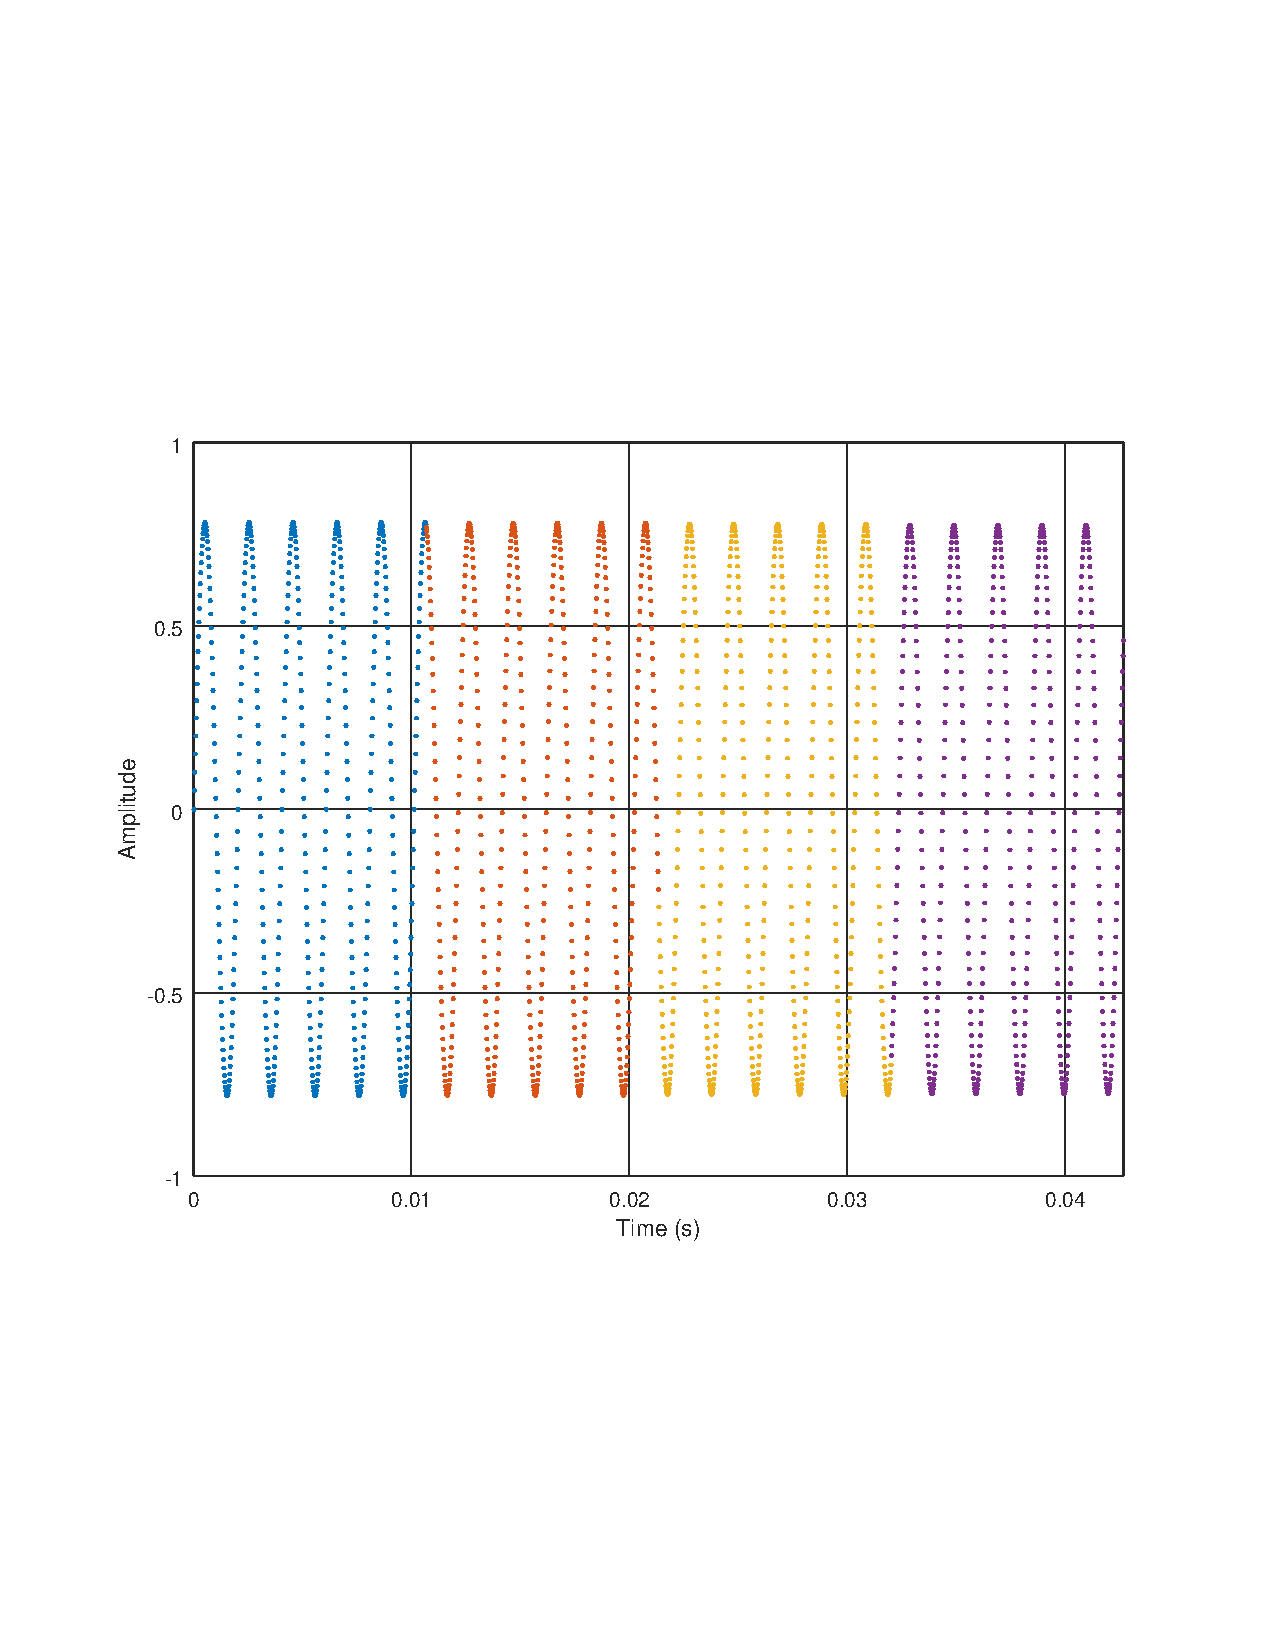
\includegraphics[width=.9\linewidth, clip, trim={2cm 7cm 2cm 7cm}]{gfx/Modelling/output.pdf}
		\caption{Output signal in the time domain. Each color represents a new block.}
		\label{fig:IFout2}
	\end{subfigure}
	\caption{Output for several following blocks, showing the phase being kept intact.}
	\label{fig:IFoutput}
\end{figure}

\FloatBarrier